% !TEX encoding = UTF-8 Unicode
\section{BLAS - Basic Linear Algebra Subprograms}
%%%%%%%%%%%%%%%%
	\begin{frame}{BLAS - Basic Linear Algebra Subprograms}
		\begin{block}{}
			\textbf{BLAS} -- specyfikacja niskopoziomowych metod działających na wektorach i macierzach.\\
			\emph{De facto} standard dla bibliotek algebry liniowej.
		\end{block}
		\begin{block}{}
			Metody podzielone na poziomy, zależnie od złożoności czasowej:
			\begin{itemize}
				\item Level-1 -- $O(n)$
				\item Level-2 -- $O(n^2)$
				\item Level-3 -- $O(n^3)$
			\end{itemize}
		\end{block}
	\end{frame}

	\begin{frame}{BLAS - dostępne operacje}
		Przykładowe operacje dla każdego poziomu:
		\begin{block}{Level 1}
			\begin{itemize}
				\item SDOT -- iloczyn skalarny
				\item SNRM2 -- norma euklidesowa
				\item SAXPY -- operacja \small $ z := \alpha * x + y $ \normalsize
			\end{itemize}
		\end{block}
		\begin{block}{Level 2}
			\begin{itemize}
				\item STRSV -- rozwiązanie równania: \small $ A * x = b $ \normalsize
				\item SGEMV -- operacja \small $ z := A * x + y $ \normalsize
			\end{itemize}
		\end{block}
		\begin{block}{Level 3}
			\begin{itemize}
				\item SGEMM -- operacja \small $ Y := A * B + C$ \normalsize
			\end{itemize}
		\end{block}
	\end{frame}

	\begin{frame}{Levels}
		\begin{enumerate}[a)]
			\item Level 1 BLAS vector-vector operations, e.g.
			$y \leftarrow y + \alpha x$
			\begin{figure}
				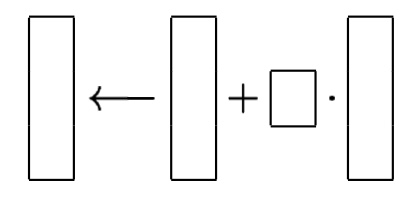
\includegraphics[height=1cm]{img/13/level1}
			\end{figure}
			\item Level 2 BLAS matrix-vector operations, e.g.
			$y \leftarrow y + Ax$
			\begin{figure}
				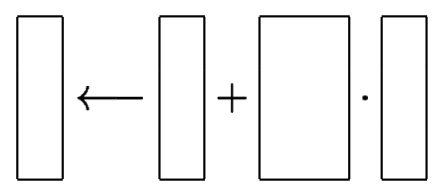
\includegraphics[height=1cm]{img/13/level2}
			\end{figure}
			\item Level 3 BLAS matrix-matrix operations, e.g.
			$A \leftarrow A + B \cdot C$
			\begin{figure}
				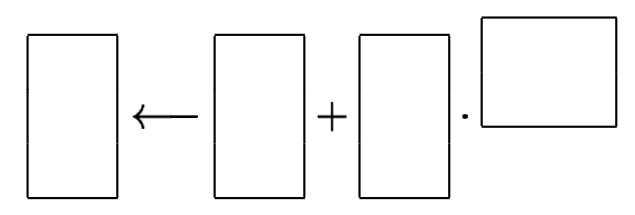
\includegraphics[height=1cm]{img/13/level3}
			\end{figure}
		\end{enumerate}
	\end{frame}

	\begin{frame}{Operacje arytmetyczne -- Hierarchia pamięci}
		Operacje arytmetyczne -- wykonywane w rejestrach, na szczycie hierarchii pamięci.
		\begin{figure}
			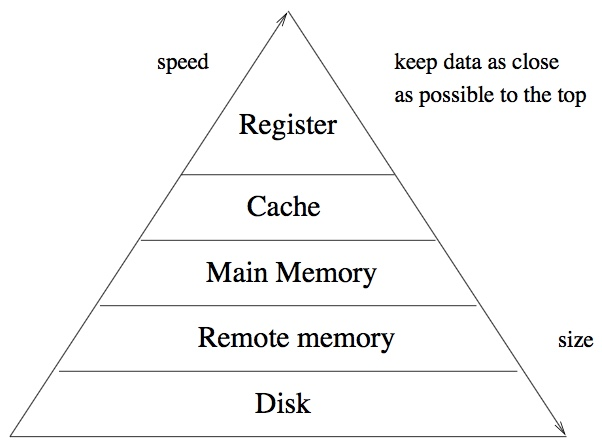
\includegraphics[height=4.5cm]{img/13/arithmeticmemref}
		\end{figure}
	\end{frame}

	\begin{frame}{BLAS -- wykorzystanie pamięci}
		\begin{block}{}
			Zwiększenie rozmiaru danych -- brak miejsca w szybkiej pamięci.\\
			\textbf{Problem: } Na kolejnych poziomach BLAS narzut czasu dostępu\\
			 do pamięci jest coraz większy.
		\end{block}

		\begin{tabular}{ | l | l | l | l | l |}
		\hline
		BLAS Level & Przykład operacji & flops 	&memref 	& $\frac{flops}{mem ref}$ \\ \hline
		1 & $y \leftarrow y + \alpha x$ 	& $2n$ 	& $3n$ 	& $\frac{2}{3} $ \\ \hline
		2 & $y \leftarrow y + Ax$ 		& $2n^2$ 	& $n^2$ 	& 2 			\\ \hline
		3 & $C \leftarrow C + AB$ 	& $2n^3$ 	& $4n^2$ 	& $\frac{n}{2}$ 	\\ \hline
		\end{tabular} \\

		\begin{block}{}
			\textbf{Przeciwdziałanie: } Zwiększenie granulacji -- zmniejszenie $n$.
		\end{block}
	\end{frame}

	\begin{frame}{BLAS -- cechy}
		Używanie BLASa zapewnia programiście szereg korzyści:
		\begin{itemize}
			\item \textit{Przejrzystość kodu} -- Możliwość skorzystania z gotowych metod, brak konieczności ich implementacji.
			\item \textit{Modułowość} -- Używanie bogatych struktur danych oraz rozbudowanych metod -- zwiększenie poziomu abstrakcji.
			\item \textit{Wydajność} -- Konkretna implementacja jest zoptymalizowana pod daną platformę.
			\item \textit{Przenośność} -- Nazwy metod są ustandaryzowane.
		\end{itemize}
	\end{frame}
	\begin{frame}{BLAS -- konwencja nazw metod}
	\[
		\underbrace{1}_{} \underbrace{2}_{} \underbrace{3}_{} \underbrace{4}_{} \underbrace{5}_{} \underbrace{6}_{}
	\]
	1 $\rightarrow$ fortran data type of the matrix \\
	2, 3 $\rightarrow$ kind of the matrix involved \\
	4, 5, 6 $\rightarrow$ type of the operation \\

	Przykład:
	\textbf{dgemm}
	\begin{itemize}
		\item d -- double
		\item ge -- general nonsymmetric
		\item mm -- matrix-matrix product
	\end{itemize}
	\end{frame}
